 %%
%% Beuth Hochschule für Technik --  Abschlussarbeit
%%
%% Hauptdokument
%%
%% 23.01.09 Tschirley V.01
%%
%%%%%%%%%%%%%%%%%%%%%%%%%%%%%%%%%%%%%%%%%%%%%%%%%%%%%%%%%%%%%%%%%%%%%
\documentclass[11pt, a4paper]{book}
%\usepackage{cite}
%% Übersetzen als Entwurf
%\usepackage[entwurf]{bhtThesis}
%% Übersetzen für die Abgabe
\usepackage[abgabe]{bhtThesis}
\usepackage[font=small,labelfont=bf]{caption}
\usepackage{mathtools}
\usepackage{multirow,tabularx}
\usepackage{graphicx}
\graphicspath{ {./img/} }
\typeout{BHT-Abschlussarbeit V.02 15.02.12 S.Tschirley}

%\usepackage{biblatex}

\usepackage{lstbayes}
\usepackage{algorithmic}
\usepackage[ruled]{algorithm2e}
\setlength\algotitleheightrule{0pt}
\SetAlgoCaptionLayout{centerline}

\makeatletter
\newenvironment{Ualgorithm}[1][htpb]{\def\@algocf@post@ruled{\kern\interspacealgoruled\hrule  height\algoheightrule\kern3pt\relax}%
\def\@algocf@capt@ruled{under}%
\setlength\algotitleheightrule{0pt}%
\SetAlgoCaptionLayout{centerline}%
\begin{algorithm}[#1]}
{\end{algorithm}}
\makeatother

\usepackage{subcaption}
\usepackage{afterpage} 
\usepackage{longtable} 
\usepackage{makecell}
\usepackage{caption}
\captionsetup[algorithm]{singlelinecheck=false}
\usepackage{pbox}
\usepackage{booktabs}
\usepackage{blindtext}   %für Blindtext in Kapitel 2
\usepackage{listings}
\usepackage{amssymb}
\usepackage{amsmath}
\usepackage{ dsfont }
\usepackage{ mathrsfs }
\usepackage{svg}

\usepackage{url}

\usepackage{color}
\definecolor{dkgreen}{rgb}{0,0.6,0}
\definecolor{gray}{rgb}{0.5,0.5,0.5}
\definecolor{mauve}{rgb}{0.58,0,0.82}


\usepackage[none]{hyphenat}
%\hyphenchar\font=-1
\sloppy

\lstset{ %
  language=R,                     % the language of the code
  basicstyle=\footnotesize,       % the size of the fonts that are used for the code
  numbers=left,                   % where to put the line-numbers
  numberstyle=\tiny\color{gray},  % the style that is used for the line-numbers
  stepnumber=1,                   % the step between two line-numbers. If it's 1, each line
                                  % will be numbered
  numbersep=5pt,                  % how far the line-numbers are from the code
  backgroundcolor=\color{white},  % choose the background color. You must add \usepackage{color}
  showspaces=false,               % show spaces adding particular underscores
  showstringspaces=false,         % underline spaces within strings
  showtabs=false,                 % show tabs within strings adding particular underscores
  frame=single,                   % adds a frame around the code
  rulecolor=\color{black},        % if not set, the frame-color may be changed on line-breaks within not-black text (e.g. commens (green here))
  tabsize=2,                      % sets default tabsize to 2 spaces
  captionpos=t,                   % sets the caption-position to bottom
  breaklines=true,                % sets automatic line breaking
  breakatwhitespace=false,        % sets if automatic breaks should only happen at whitespace
  title=\lstname,                 % show the filename of files included with \lstinputlisting;
                                  % also try caption instead of title
  keywordstyle=\color{blue},      % keyword style
  commentstyle=\color{dkgreen},   % comment style
  stringstyle=\color{mauve},      % string literal style
  morekeywords={*,...}            % if you want to add more keywords to the set
} 




%%\usepackage{hyperref}

%\usepackage[round]{natbib}

%%
%% Es folgen einige Zusätze, die in Kapitel 1 beschriben sind. 
%% Alles was nicht notwendig ist, kann auskommentiert werden
%%
\usepackage{trsym}
%\usepackage{showkeys}
\usepackage{bytefield}

\def\blankpage{%
      \clearpage%
      \thispagestyle{empty}%
      \addtocounter{page}{-1}%
      \null%
      \clearpage}

%%
%% Pfad zu den Bildern
%%
\graphicspath{
  {img/},
}

%%
%% Einbinden persönlicher macros 
%%
%
% Persönliche Macros
%
%

% Macros für Formeln
\newcommand{\jw}{j\omega}

% Begriffe

\newcommand{\OPV}{Operations\-ver\-stär\-ker}



%% Message
\typeout{-----------------------------------------------------------}
\typeout{----> main.tex ---- Zentrales Dokument---------------------}
\typeout{-----------------------------------------------------------}

\version{0.1$\alpha$}
\datum{\today}
%%
%% Titel, Autor und Betreuer
%%
\fachbereich{VI} 
\studiengang{Medieninformatik}
\autor{Sebastian Herrmann}
\edvnr{852049}
\titel{Generating Electronic Health Records: an Investigation on Gender-Medicine and Rare Diseases}
%\untertitel{Evaluating the Accuracy of Variational Bayes Variational Inference in Survival Analysis}
\betreuerFeld{
  \begin{tabular}{lr}
    \multicolumn{2}{l}{\textbf{Gutachter}}\\
    Prof. Dr.-Ing. habil. Alexander Löser & Beuth Hochschule für Technik Berlin\\
    Prof. Dr. Felix Bießmann & Beuth Hochschule für Technik Berlin
  \end{tabular}
}

%%%%%%%%%%%%%%%%%%%%%%%%%%%%%%%%%%%%%%%%%%%%%%%%%%%%%%%%%%%%%%%
%% Literaturverzeichnis

\clearpage\newpage
\addcontentsline{toc}{chapter}{References}

%\bibliographystyle{apa}
%\bibliography{library}
\usepackage[style=apa,backend=biber]{biblatex}

\addbibresource{library.bib}


%%\renewcommand{\baselinestretch}{1.05} 
\begin{document}
\pagestyle{fancy}
%\thispagestyle{empty}
\renewcommand{\bibname}{References}

%makecell package formatting
\renewcommand\theadfont{\normalsize}
%\renewcommand\theadfont{\itshape}

\thispagestyle{empty}
\maketitle

\blankpage

\thispagestyle{empty}
\section*{Abstract}
XXX


\blankpage

\clearpage

\thispagestyle{empty}

%----------------------------------------------------------------------------------------
%	LIST OF CONTENTS/FIGURES/TABLES PAGES
%----------------------------------------------------------------------------------------

\tableofcontents % Prints the main table of contents

\listoffigures % Prints the list of figures

\listoftables % Prints the list of tables

\clearpage

%----------------------------------------------------------------------------------------
%	ABBREVIATIONS
%----------------------------------------------------------------------------------------
\begin{abbreviations}{ll} % Include a list of abbreviations (a table of two columns)

\textbf{GAN} & \textbf{G}enerative \textbf{A}dversarial \textbf{N}etwork\\
\textbf{medGAN} & \textbf{med}ical \textbf{G}enerative \textbf{A}dversarial \textbf{N}etwork\\
\textbf{G} & \textbf{G}enerator}\\
\textbf{D} & \textbf{D}iscriminator\\
\textbf{CAD} & \textbf{C}oronary & \textbf{A}rtery & \textbf{D}isease\\
\textbf{CVD} & \textbf{C}ardio\textbf{v}ascular & \textbf{D}isease\\
\textbf{DM} & \textbf{D}iabetes & \textbf{M}ellitus
\end{abbreviations}


\pagenumbering{arabic}
%%%%%%%%%%%%%%%%%%%%%%%%%%%%%%%%%%%%%%%%%%%%%%%%%%%%%%%%%%%%%%%





\chapter{Introduction}
% Am Anfang jedes Kapitels kurze Übersicht, was das Kapitel beinhaltet

\section{Artificial intelligence in health care}
Artificial intelligence (AI) tries to simulate human intelligence. Its applications are numerous and can also be found in the health care sector. A possible use case could be an assisting AI system, that provides up-to-date information about clinical practices to physicians and reduces errors, in therapeutic and diagnostic context. \cite{jiang2017artificial}. Electronic health records (EHR) are the digital version of a patient's medical healthcare information over a lifetime. AI can extract and analyze patient data from such records and give alerts for possible health risks and, e.g. make predictions about diagnoses and the possible length of stay in the hospital. \cite{neill2013using}. Practically such a system could analyze a patient's data already during reception and provide a first diagnosis. Another exemplary use case is the application of AI in diagnosis for breast cancer detection. \cite{ubeyli2007implementing} Despite the many use cases, publicly available EHR data for research is rare. This is mainly to protect each patient's privacy. However, this especially poses a problem to the availability of data about rare diseases, leading to a lack of information and slowing down research. \cite{bremond2015contribution}

\subsection{Generative Aversarial Networks}
Since their introduction in 2014 by \cite{Goodfellow2014}, Generative Adversarial Networks have gained a substantial extent of attention. This is mainly due to their ability of augmenting synthetic image data that can not be distinguished from real data. This quality proofs to be useful in the medical domain and to its applications count for example the augmentation of medical images of liver lesions. These images can be used to train and to improve the performance of a convolutional Neural Network that classifies liver lesions. \cite{frid2018gan} Explained briefly, a GAN consists of two neural networks, that are playing against each other. One creates fake samples, while the other one tries to distinguish these samples from real ones. During this process, both networks train each other. \citep{Goodfellow2014} Its functionality will be explained in detail in the following Chapter 2.

\section{Goal}
The aim of this work is to generate EHRs. For generation we use a approach by \cite{Choi2017} which produces high-dimensional discrete variables (e.g., binary and count features) using an altered Generative Adversarial Network, called medical Generative Aversarial Network (medGAN). As input dataset we use an EHR dataset called MIMIC-III. In contrast to the model presented in \citep{Choi2017}, we additionally split the input dataset by gender.
 We want to investigate, whether the samples the medical Generative Adversarial Network (medGAN) generates will be more realistic, by splitting the input data by gender. Further, we want to investigate whether medGAN is able to generate realistic samples with rare diseases.
 
\section{Method}
In our research we use the same model as already mentioned in \cite{Choi2017}. We change the input training data, by spitting up the data by gender. Subsequently, we train the network, using both, binary and count variables. We train the model with the full dataset and afterwards with the dataset of each gender. First, we evaluate our measurements in a quantitative manner, using dimension-wise probability for binary output und dimension-wise average for count output. KS TEST? In our qualitative evaluation, we investigate our measurements for a correlation of Cardiovascular Disease (CVD) and Diabetes Mellitus (DM). Further, we will evaluate our measurements with the help of a medical doctor.

\subsection{MedGAN}
A central aspect of this work will be the application of the medical Generative Adversarial Network (medGAN), that is proposed by \cite{Choi2017}.
It is a GAN, able to generate realistic synthetic patient records, that achieve comparable results to real data when used for predictive modeling tasks. \cite{Choi2017} proof in their work, that medGAN outperforms classical machine learning algorithms like Linear Regression, Random Forests and Support Vector Machine. 
In Chapter 2, the motivation of creating medGAN will be explained. In Chapter 4, we will provide detailed information on the architecture of medGAN and will elaborate on recent improvements on medGAN.
\subsection{Generating binary and count features}
For our experiments, we generated both, records with binary and count variables. Records with binary data will show whether an ICD-9 code occured or not, \textbf{Table 1.1} shows exemplary data. Records with count data will show how many times each ICD-9 code occurred for each patient, as depicted in \textbf{Table 1.2}
\\
\\

\begin{table}
\begin{center}
\begin{tabular}{l*{3}{c}r }
Patient ID & 272 & 414 & 780 \\
\hline
A & 0 & 0 & 1 \\
B & 1 & 1 & 0 \\
C & 0 & 0 & 0 \\
\hline
\end{tabular}
\caption{Example binary data entries with 3 digit ICD-9 codes}
\label{tab:example-binary}
\end{center}
\end{table}


\begin{table}
\begin{center}
\begin{tabular}{l*{3}{c}r }
Patient ID & 488.11 & 516.30 & 996.49 \\
\hline
A & 0 & 5 & 0 \\
B & 1 & 0 & 9 \\
C & 0 & 2 & 0 \\
\hline
\end{tabular}
\caption{Example count data entries with 5 digit ICD-9 codes}
\label{tab:example-count}
\end{center}
\end{table}

\subsection{Privacy Risk}
The risk of hurting a patient's privacy is one of the main reasons why Electronic Health Data is not publicly available. A commonly used method for providing access to patient data for researchers is de-identification, used, for example, on the MIMIC-III dataset. In this process, data gets cleansed and shifted, meaning that names, telephone numbers, and other personal informations get removed and dates altered. \cite{johnson2016mimic}
However, \cite{Choi2017} explains that de-identification does not eliminate the risk of harming a patient's privacy, because identification of an individual is still possible, if an attacker has information about, e.g. diagnoses, lab tests, demographics, genomic variants or visits from other health care providers.

On the contrary, as the synthetic data from medGAN is artificially created, there is no direct connection between the real and the synthetic samples. Therefore identifying patients from the original dataset should, intuitively, not be possible if the artificially created samples get stolen because of a security breach or due to other reasons. In \cite{Choi2017} assesses the privacy risk for the case that the synthetic samples get compromised and comes to the conclusion that a potential attacker poses no risk of breaching privacy, except for when he already has significant knowledge about various features of the target patient.

\section{Outline}
This work is divided into 6 chapters, starting with 'Introduction.', where we learned about the application of AI in health care, Generative Adversarial Networks and the extended version, medGAN, that we will apply in our work. In the next chapter 'Related Work', we will dive deeper into the topic by explaining all the essential concepts that will be used in our research. In Chapter 3,  'Data Analysis', we will analyze the given MIMIC-III dataset. Subsequently, in Chapter 4, 'Electronic Medical Record Generation', we will perform our experiments and generate the EHR data. Afterwards, in 'Experimental Evaluation', we will assess the success of our experiments. Lastly, in Chapter 6 'Conclusion and Outlook', we will conclude whether our hypotheses held up during our experiments and will give an outlook on possible future work.

\section{Summary}
This chapter explained the motivation for using AI in the medical sector and reason for scarcity of data in this field. For giving an insight into our method, we first provided a short definition of Generative Adversarial Networks and medGAN. GANs will be more thoroughly explained in the following Chapter 2, medGAN in Chapter 4. This chapter also depicts two examples of the representation of the generated data. We also addressed \cite{Choi2017}'s work on investigating the privacy risk that synthetic samples pose.

\chapter{Related Work}
\section{Abstract}
The following section will elaborate on the basic concepts that are needed to  generate synthetic electronic health record data.
First, we explain the concept of a Generative Adversarial Network. Further, we will define what exactly an Electronic Health record is. Subsequently, we will introduce the definition of Gender Medicine and Rare Diseases and their role in this work. Lastly, we will give information on medGAN and thoroughly explain its characteristics and architecture in Chapter 4.

\section{Basic Concepts}
\subsection{Generative Adversarial Networks}
In \cite{goodfellow2014generative} proposed a new framework for generative models, that learns the patterns in a given dataset and generates new data that plausibly could originate from the original dataset.
 The model \cite{Goodfellow2014} proposes corresponds to a two-player minimax game: in which two independent neural networks train simultaneously. The generator \textbf{G} tries to learn the distribution of the given dataset and the discriminator \textbf{D} aims to distinguish between the data from the training set and from \textbf{G}. \textbf{G} generates the data from the learned distribution and takes random noise as input. In this game, G has the goal to maximize the probability of D making a mistake.  
\\
\\
The two-player minimax game, as shown in \cite{Goodfellow2014}, can be described by the following value function:
\\
\begin{equation}
	\min_G\max_DV(D,G) = \mathbb{E}_{x\sim{P_{data(x)}}}[log D(x)] + \mathbb{E}_{z\sim_{P_z(z)}}[log(1 - D(G(z)))]
\end{equation}
\\

For a better understanding of the process of the model, the following analogy can be helpful:
"The generative model can be thought of as analogous to a team of counterfeiters, trying  to  produce  fake  currency  and  use  it  without  detection,  while  the  discriminative  model  is analogous to the police, trying to detect the counterfeit currency.  Competition in this game drives both teams to improve their methods until the counterfeits are indistinguishable from the genuine articles." \cite{goodfellow2014generative}

Mainly due to their performance in generating synthetic image data that can not be distinguished from real images, Generative Adversarial Networks gained a considerable amount of attention since their introduction in 2014.


% minGmaxDV(D,G) =Ex∼pdata(x)[logD(x)] +Ez∼pz(z)[log(1−D(G(z)))].
\subsection{Electronic Health Records}
The Healthcare Information and Management Systems Society defines an Electronic Health Record as "a longitudinal electronic record of patient health information generated by one or more encounters in any care delivery setting. Included in this information are patient demographics, progress notes, problems, medications, vital signs, past medical history, immunizations, laboratory data and radiology reports." \cite{HIMMS}
The term 'Electronic Medical Record' often is used synonymously, but a distinction between both terms has to be made.
The Office of the National Coordinator for Health Information Technology defines an EMR as the digital version of a patient's paper record. It contains time tracking data, health parameters (for example blood values), and information about checkups. They are maintained for each practice. It's intended usage is for the hospital or doctor itself and it is not meant to be shared. \cite{ONC}
EHRs, on the other hand are meant to give a perspective on the overall health of each patient and to be shared for research, other healthcare providers and even the patients themselves. They contain a patient’s life-long medical history, medications, diagnoses, treatment plans, vaccination dates, allergies, images, laboratory data (e.g. blood values) and test results. \cite{ONC} A problem with EHR data, is that interoperability is not always given due to missing standardization. \cite{johnson2016mimic}
In our work we will focus on generating diagnoses codes. MedGAN is also able to generate medication and procedure codes.

\subsection{Gender Medicine}
Medical research is dominated by the male gender, meaning that women are heavily underrepresented or sometimes even excluded from research studies not only in animal studies but also in human trials. \cite{baggio2013gender} 
But diseases differ between genders, not only in terms of prevention but also in clinical signs and therapeutic approach  \cite{baggio2013gender}
Sex-differences can also be found in the correlation of diseases. \cite{kautzky2010sex} shows in his research that "Sex-specific differences appear particularly relevant in the management of type 2 diabetes mellitus (T2DM), with women experiencing greater increases in cardiovascular morbidity and mortality than do men." \cite{kautzky2010sex}
Gender, however, does not only include sex, but also lifestyle-related diseases, stress, and behaviour, like, for example, regarding help-seeking actions.
While we can not take the socio-cultural aspect of gender into account, the differences in sex are applicable.
As "cardiovascular disease is the leading cause of death of both men and women" \cite{arain2009sex}, we can find numerous occurrences in the MIMIC-III dataset. This allows us to investigate the co-occurrences of \textit{Diabetes Mellitus (DM)} and \textit{Cardiovascular Disease (CVD)}.
Originally MedGAN was trained with male and female patients simultaneously, making no difference between them. In this work we are separating the dataset in order to introduce a distinction between genders.

The previously mentioned gender-differences lead us to one of our hypotheses, that by training the network with samples of each gender separately, its performance improves and it is able to generate patients with gender-specific correlated diseases that seem realistic to a medical doctor.

\subsection{Rare diseases}
In Europe, a rare disease, also known as orphan disease, is defined as such when there are no more than 5 occurrences in 10.000 people. As defined by Orphanet, there are roughly 6,000 to 7,000 rare disorders, which include diseases, syndromes and anomalies. The characteristic of a disease is an altered state of health, presented "as a unique pattern of symptoms with a single treatment". \cite{Orphanet}. The majority of rare diseases have a genetic origin, but can also originate from an infection or due to unknown reasons. \cite{Orphanet} Specific codes for orphan diseases are only scarce in international classification systems like ICD-9 or ICD-10, which is used in this work, resulting in a deficit of information  for researchers regarding orphan diseases. This problem finds its cause in the lack of research and a lack of awareness for rare diseases until recently, also resulting in patients without a diagnosis and unidentified illnesses. \cite{Orphanet}
Therefore Orphanet developed a nomenclature, in which each rare disease receives a unique ORPHAnumber. Access to the Orphanet classification system is provided through their website\footnote{https://www.orpha.net/}. This system increases visibility of rare diseases and interoperability among health and research information systems. \cite{Orphanet}




\subsection{medGAN}
The wide adoption of the electronic health record system by healthcare organizations (HCOs) promises advances in analyzing patient data and computational health. The records, however, are not easily accessible for researchers. Due to the fact that EHR data consists of personal and sensitive information, access is restricted in order to not induce a privacy risk. Further, to minimize the risk of data misuse, access to such data is regulated by the HCOs. \cite{Choi2017}
(Even researches that are in direct cooperation with a hospital, do not get access to patient data.)
 As \cite{Choi2017} states, the process of getting access is a time-consuming act and without guarantee to gain it. The restricted access slows down research. )." \cite{Choi2017} further describes, that despite processes like date-shifting and alteration and randomization of personal  information, a patients are still prone to re-identification. "To generate synthetic data (McLachlan et al., 2016; Buczak et al., 2010; Lombardo and Moniz, 2008)" \citep{Choi2017}, also does not solve the problem, as the resulting data is not sufficiently realistic to be used as training data.
 To overcome the limitations and risks of the above-stated methods, \cite{Choi2017} introduced medGAN, which implements a Generative Adversarial Network that leverages an autoencoder to overcome its limitations: the GAN generates distributed representations of patient records, while the autoencoder decodes them into actual discrete records.
 This principle and the detailed architecture of medGAN will be further explained in the section 'Electronic Medical Record Generation'.

\section{Summary}
This chapter provided an overview of fundamental concepts that need to be understood to generate electronic medical records and to evaluate our measurements.
It gave an insight into Generative Adversarial Networks, and how they will be used in this work and into the definition of Electronic Health Records and how they are distinguishable from Electronic Medical Records.
The chapter proceeded with an explanation of gender-medicine and rare diseases and their role for the evaluation process in Chapter 5. It concluded in a detailed explanation of medGAN, that will be used in Chapter 4. In the following Chapter 3, we will investigate the MIMIC-III dataset.

\chapter{Dataset and Analysis}
\subsection{Abstract}
In this Chapter, we will learn about the MIMIC-III dataset, how it is structured and what contents it includes. Afterwards we will investigate the dataset for the most frequent diagnosis codes and give an overview about the correlation of diseases in the dataset. Further we will give a look at the co-occurrence  of DIabetes Mellitus (DM) and Cardiovascular Disease (CVD) for female and male patients.

\subsection{Dataset}
The MIMIC-III ('Medical Information Mart for Intensive Care') dataset is one of the biggest publicly available in the medical domain. It is developed and maintained by the MIT lab for computational physiology. It comprises de-identified health data of approximately 45,000 patients admitted to critical care units at Beth Israel Deaconess Medical Center in Boston. The data includes information such as vital signs, procedure codes, diagnostic codes, medications, laboratory measurements, observations, fluid balance, length of stay, survival data, and more. 
\begin{figure}
  \begin{center}
  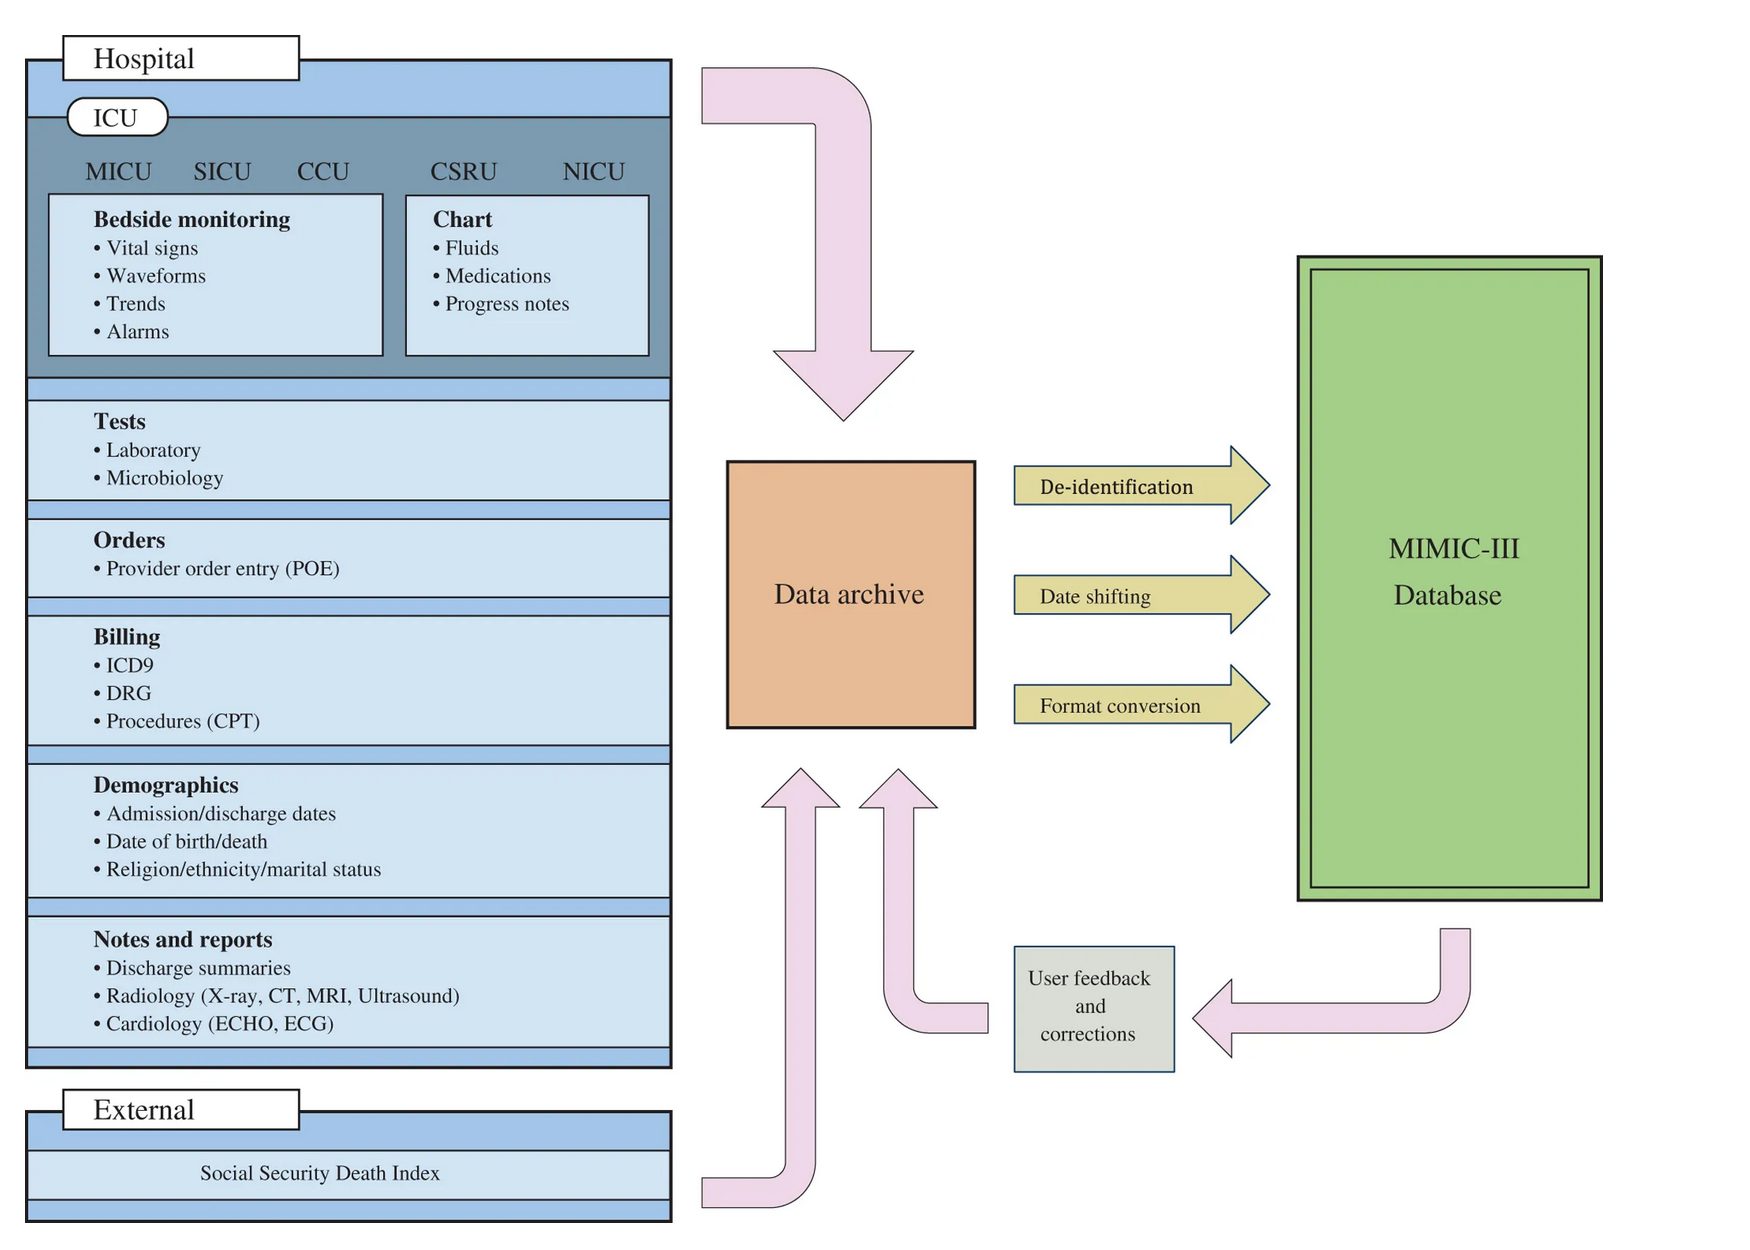
\includegraphics[width=1\textwidth]{img/mimicIII-schema.png}
  \caption{Schematic overview over MIMIC-III \cite{NAT}}
  \label{fig:mimic-III-schema}
  \end{center}
\end{figure}

\textbf{Figure 3.1} depicts the schema of MIMIC-III. On the left, in the blue section, we can see the data that the Beth Israel Medical Center collects. This data is stored in an archive. After applying de-identification, date shifting and format conversion, the EHR data gets into the MIMIC-III database, which is maintained and updated with the help of user feedback by the team of 'The Laboratory for Computational Physiology at Massachusetts Institute of Technology' (MIT) \cite{johnson2016mimic}
\subsection{Analysis}

Before conducting our research we performed an exploratory data analysis on the MIMIC-III dataset. The goal of this analysis was to discover patterns and correlations in the data to formulate hypotheses for further analysis. We used pandas and numpy for the analysis and matplotlib, to display the results. The total number of unique patients found in the dataset is 46520, consisting of 26121 male and 20399 female patients.


\begin{table}
\begin{tabularx}{\textwidth}{X|l|r|r|r}
ICD Code & Diagnosis & Frequency & Patients affected & \% of associated patients \\
\hline
401.9 & Essential hypertension & 20703 & 17613 & 37.86\\
414.01 &  Coronary atherosclerosis & 15229 & 13480 & 28.98 \\
428.0 & Congestive heart failure &   13111 & 9843 &21.16\\
427.31 & Atrial fibrillation&    12891 & 10271 &  22.08\\
584.9 &  Acute kidney failure &  9119 & 7687& 16.52\\
250.00 & Diabetes mellitus &  9058 & 7370 & 15.82\\
272.4 & Unspecified hyperlipidemia & 8690 & 7465 & 16.05 \\
518.81 &  Acute respiratory failure & 7497 & 6719 & 14.04 \\
599.0 &   Urinary tract infection &  6555 & 5779 & 12.42 \\
530.81 & Esophageal reflux &  6326 & 5272 & 11.33\\
\end{tabularx}
\caption{\label{tab:top10-codes-dataset}Top 10 of most occurring ICD-9 codes in the dataset}
\end{table}


First, as a basic overview, we check for the Top10 most occurring ICD-9 codes in the dataset. As depicted in \textbf{Table 3.1}, \textit{essential hypertension} has the highest frequency in MIMIC-III, followed by 3 more codes of circulatory diseases. \textit{Diabetes mellitus (DM)} can also be found in the list of the most occurring codes.

\begin{figure}
  \begin{center}
  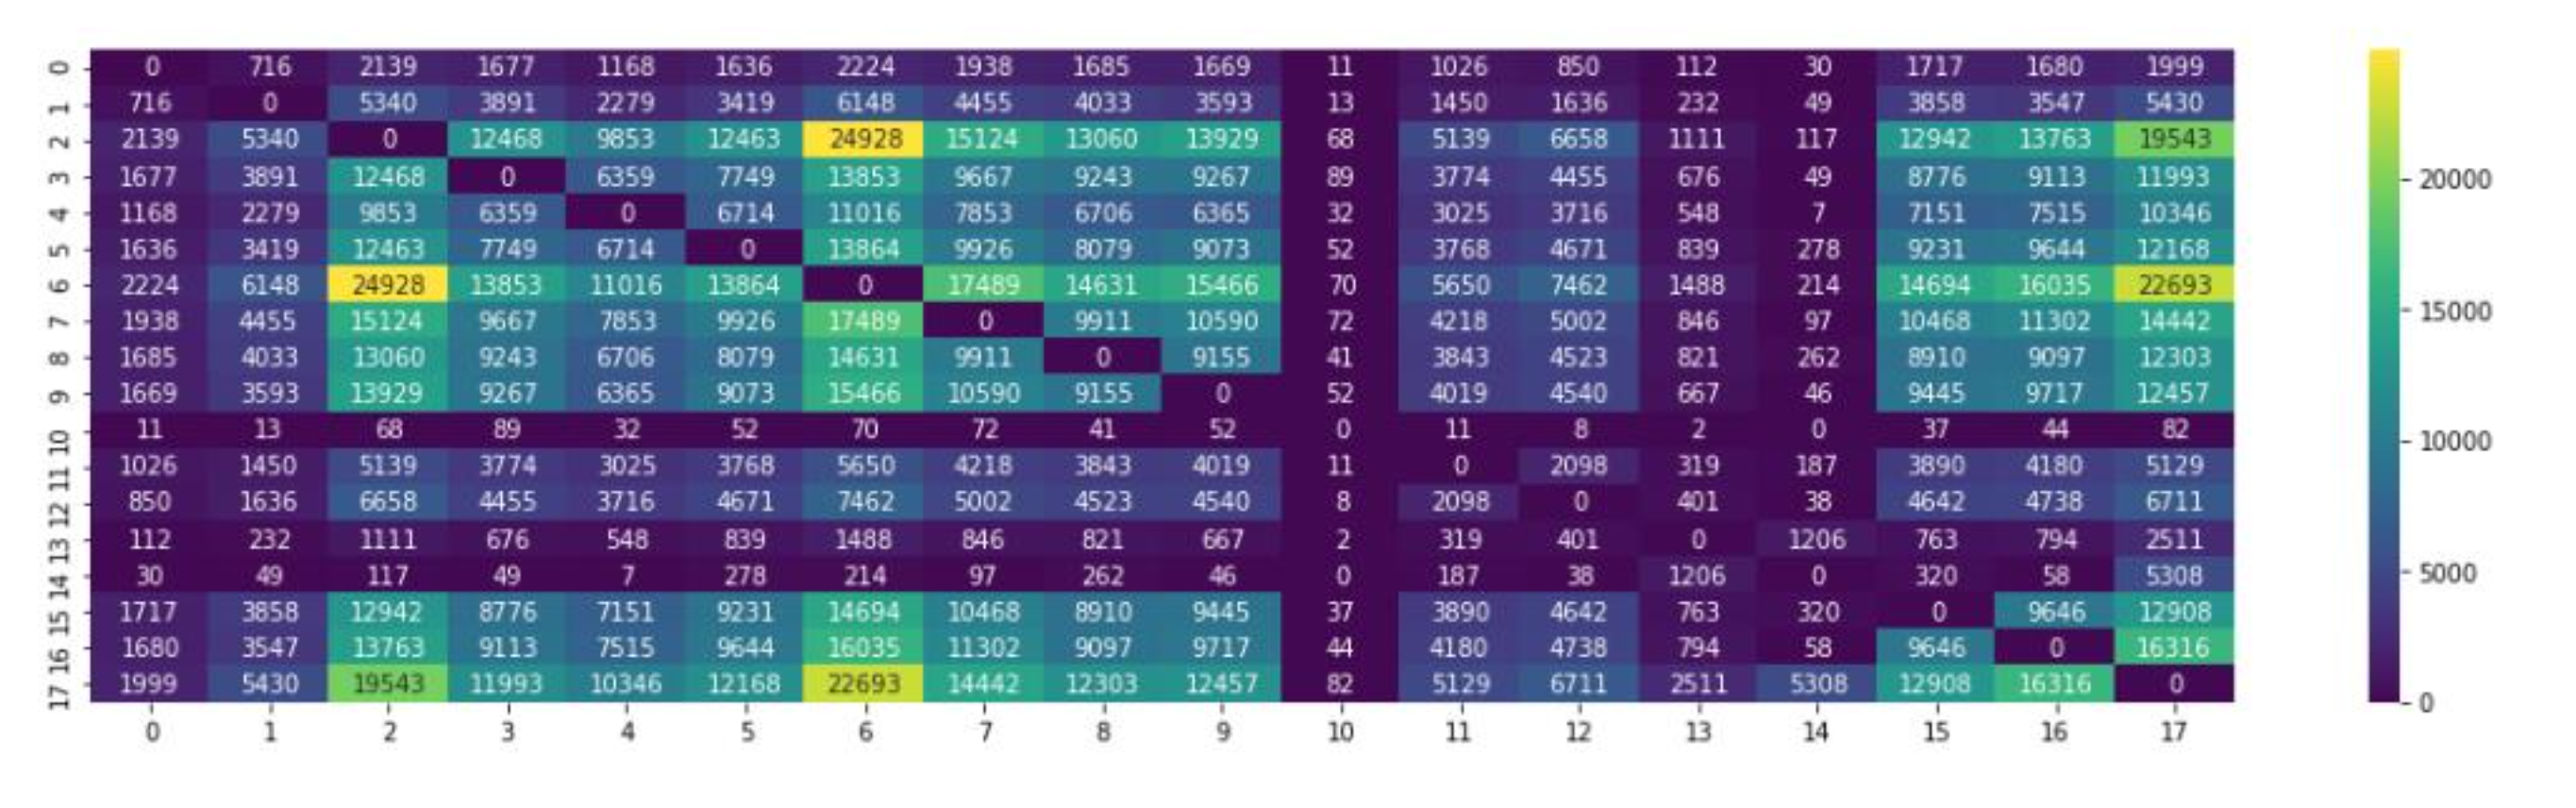
\includegraphics[width=1\textwidth]{img/correlation-heatmap.png}
  \caption{Correlation heatmap of ICD code groups \cite{arya2019exploratory}}
  \label{fig:correlation-heatmap}
  \end{center}
\end{figure}


\\
\\
Next, we have a look at the correlation heatmap (\textbf{Figure 3.2}) that is introduced in \cite{arya2019exploratory}. In this map, ICD-9 codes are divided into 18 groups. It shows, how many patients have a diagnosis of two groups at a same time and compares every group to each other. It shows the strongest correlation of ICD-9 codes from the groups two and six, which correspond to \textit{endocrine, nutritional and metabolic diseases and immunity disorders} and \textit{diseases of the circulatory system}. Codes from group two refer to the range of codes from 240-279 , codes from group six refer to codes in the range from 390 to 459. As shown in \textbf{Table 3.1}, codes from group six are the most frequent. From group two, we can find two codes, 250.00 \textit{Diabetes mellitus} and 272.4, \textit{unspecified hyperlipidemia}.
\\

Subsequently, we filter all patients with coronary artery disease (Code 414.01) by diabetic diseases (Code 250.*) and compare the frequencies for male and female patients. 7280 female and 9174 male patients are affected by any form of diabetic disease.
For coronary artery disease, 3660 female and 9820 male patients are affected. 


\begin{table}
\begin{center}
\begin{tabularx}{\textwidth}{X|r|r|r|r}
Gender & diabetes & no diabetes & Total & Percentage\\
\hline
Female & 1518 & 2142 & 3660 & 41.48\%/58.42\%\\
Male 	& 2705 & 7115 & 9820 & 27.55\%/72.45\%\\
\end{tabularx}
\caption{\label{tab:cad-diabetic}Patients that have CAD and diabetes and patients, that have CAD and no diabetes}
\end{center}
\end{table}


In \textbf{Table 3.2} we can see, that female patients with diabetic disease are significantly more often affected by coronary artery disease than male patients. The increased prevalence of cardiovascular diseases for women that have DM is a known risk factor, as already stated in Chapter 2.


\section{Summary}
This chapter gave an insight into the distribution of female and male patients and the most frequent ICD-9 codes in the MIMIC-III dataset. We also learned that statistically, significantly more female patients are affected by coronary artery disease if they also have diabetic disease. This correlation can not be found in male patients.  
In our qualitative evaluation in Chapter 5, we will verify whether our model is able to reproduce these co-occurrences.

\chapter{Electronic Health Record Generation}
\section{Abstract}
In this chapter, we will elaborate medGAN, and explain how it differentiates to a traditional GAN. Moreover we will give an insight into recent improvements of medGAN and its different version. Further, we will discuss the process of training and generating synthetic Electronic Health Record data on the cloudservice 'Colaboratory' and explain the architecture of medGAN, and our experimental setup. Also, we will introduce our hypotheses and describe, how we used the data of the MIMIC-III dataset.
\section{medGAN}
One part of medGAN is a GAN, which consists of two independent neural networks that train each other. The first one is the \textit{Generator (G)} that creates the synthetic data and presents it to the second one, the \textit{Discriminator (D)}. During training real and synthetic samples are presented to \textbf{D}, which tries to distinguish between both.
\textbf{D} and \textbf{G} are both implemented as feedforward neural networks.
As we learned in 2.2.1, the generator \textbf{G} "is trained by the error signal from the discriminator D via backpropagation, the original GAN can only learn to approximate discrete patient records $x \in Z|C|$ with continuous values. ” \cite{Choi2017}
To alleviate this limitation, they leveraged an autoencoder which is reconstructing an dimensionality reduced approximate of the input. As \cite{Choi2017} explains, that during this process, the autoencoder learns the unique features of the samples and that this mechanism has previously been used on image processing tasks.

"The objective of the autoencoder is, to minimize the reconstruction error:

\begin{equation}
\frac{1}{m}\big[\sum_{i=0}^m \mid\mid x_i - x_i'\mid\mid_2^2]
\end{equation}
\begin{equation}
\frac{1}{m}\big[\sum_{i=0}^m x_i \log x'_i + (1-x_i) \log (1-x'_i)]
\end{equation} 
\begin{center}
where $x'_i = Dec(Enc(x_i))$
\end{center}

where m is the size of the mini-batch." \cite{Choi2017}
\\
\\
An autoencoder consists of of two elements: The Encoder (\textit{Enc}) which compresses the input and the Decoder (\textit{Dec}) that is used to construct the output.
%For count variables they used the \textit{cross entropy loss} and \textit{rectified linear units (ReLU}  as activation function for the \textit{Enc} and \textit{Dec}.
For binary variables they used the \textit{mean squared loss} and the \textit{tanh} activation function for \textit{Enc} and the \textit{sigmoid} activation for \textit{Dec}.
Both, the \textit{Enc} and the \textit{Dec} are implemented as single-layer feedforward networks. The original input x it receives, is compressed into a 128 dimensional vector. The generator \textit{G} consists of two hidden-layers with each 128 dimensions and is implemented as a feedforward network. For the batch normalization in \textit{G} they use the scale parameter  $\gamma$ and the shift parameter $\beta$ and set the moving average decay to 0.99. The discriminator \textit{D} inherits the same structure, but the first hidden-layer consists of 256 dimensions. MedGAN is trained for 1,000 epochs with the mini-batch of 1000 records. \cite{Choi2017}
\begin{figure}
  \begin{center}
  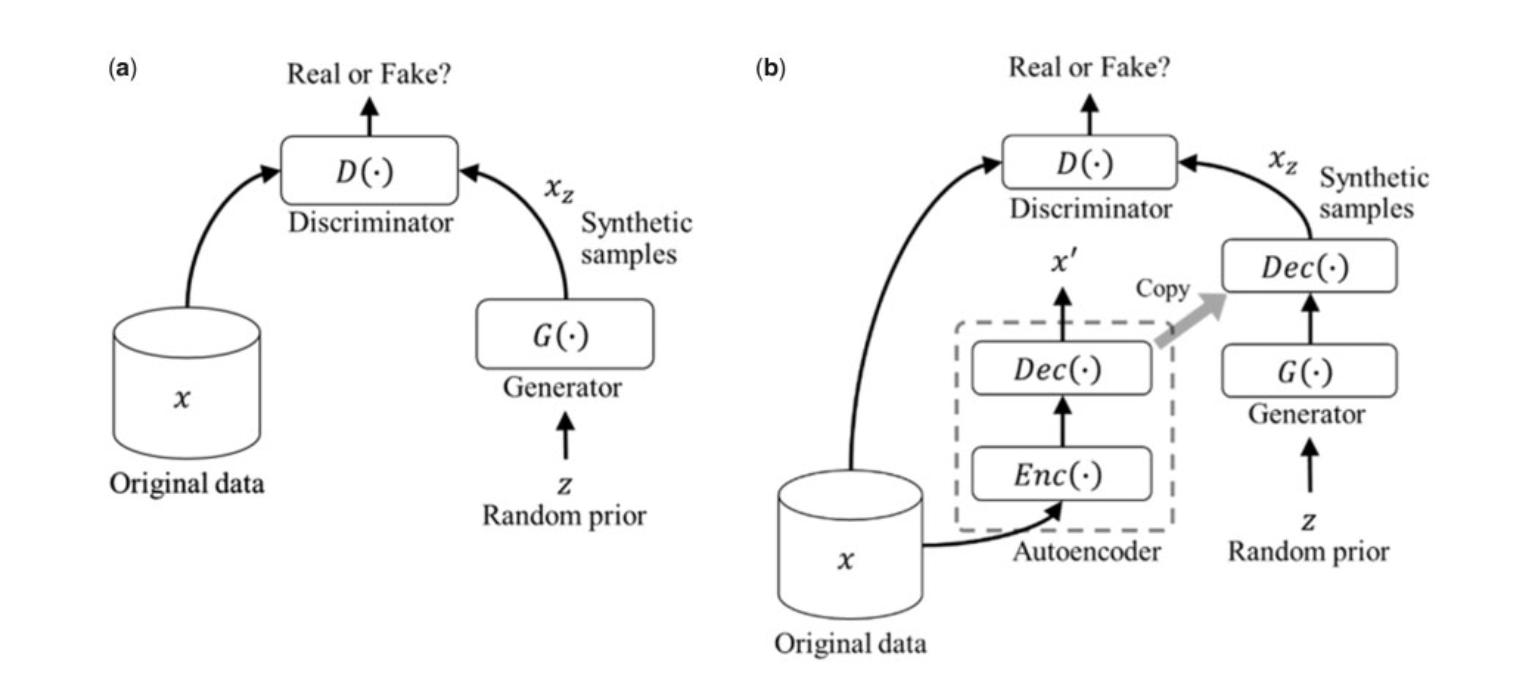
\includegraphics[width=1\textwidth]{img/ganVSmedgan.png}
  \caption{Architecture of traditional GAN \textbf{(a)} and medGAN \textbf{(b)}: The discrete x comes from the source EHR data, z is the random prior for the generator G; G is a feedforward network with shortcut connections (right-hand side figure); An autoencoder (i.e, the encoder Enc and decoder Dec) is learned from x; The same decoder Dec is used after the generator G to construct the discrete output. The discriminator D tries to differentiate real input x and discrete synthetic output Dec(G(z)).  \cite{Choi2017}} Figure from \cite{Baowaly2018}.
  \label{fig:medgan-architecture}
  \end{center}
\end{figure}

One of the key underlying problems of GANs is \textit{mode collapse}. \textit{Mode collapse} happens, when the generator learns a single or a few samples that the discriminator accepts and keeps generating the same sample(s).
\cite{Choi2017} approaches the problem of mode collapse, by introducing \textit{minibatch averaging}, which functions similarly to \textit{minibatch discrimination}. The general idea is that during training, \textit{D} sees the minibatch of real samples during classifying fake samples and vice-versa.
While minibatch discrimination compares the calculated distance of each given sample and the samples of the minibatch, minibatch averaging calculates the average of the samples in the minibatch. In contrast to minibatch discrimination, minibatch averaging does not require any additional parameters and therefore its impact on the training time is neglectable. \cite{Choi2017}
Additionally, batch normalization and shortcut connection need to be applied, to increase the learning efficiency of \textbf{G}. Otherwise \textbf{D} will overpower \textbf{G}. \cite{Choi2017}

\subsection{SynthEHR (medBGAN, medWGAN)}
Recently, \cite{Baowaly2018} proposed two altered versions of medGAN that outperform their predecessor, however just slightly.
\\
Those two versions are:
\textbf{medWGAN}: This version substitutes the regular GAN with an improved \textit{Wasserstein GAN (WGAN)}, that utilizes "an alternative method of weight clipping called gradient penalty, which entails penalizing the norm of the gradient of the discriminator (critic) with respect to its input" \cite{Baowaly2018}

\textbf{medBGAN}: This version substitutes the regular GAN as well, but this time with a \textit{boundary-seeking GAN (BGAN)}. This approach trains the generator to match the target distribution that converges toward the true distribution as the discriminator is optimized" \cite{Baowaly2018}
\subsection{Differentiation}
MedWGAN and medBGAN both learn interdimensional relationships better than medGAN. We are trying to proof, that medGAN will improve on this point, if trained with female and male patients separately.
If our hypotheses proof to be true and bring an improvement to medGAN, these improvements will also translate to altered versions of medGAN, because not the network itself is being changed but the input. In our tests we separated the dataset and did not alter it. Henceforth we performed our tests only on the 'original' medGAN. 
\section{Process and Architecture}
For generating the Electronic Medical Records (EMR), we used a Generative Adversarial Network (GAN) called medGAN, that was proposed in \cite{Choi2017}. As input data we use v1.4 of the MIMIC-III (Medical Information Mart for Intensive Care) dataset. We train the model with full-length ICD-9 codes, that are 5 digits in length. Additionally, we train the model with generalized ICD-9 codes, that are 3 digits long. For our experiments, we divided the dataset by gender and generated EMR data with binary and count variables for both mixed and separated patients. The code for medGAN is publicly accessible under https://github.com/mp2893/medgan. It is implemented using TensorFlow.
For training models, they chose the Adam-optimizer with a mini-batch size of 100 patients. \cite{Choi2017} We trained the model using Colaboratory by Google\footnote{colab.research.google.com/}, which is a Jupyter notebook environment, providing free Cloud computing for education and research.
The machine is equipped with a Tesla T4 GPU from NVIDIA.

\begin{table}
\begin{center}
\begin{tabularx}{\textwidth}{X|r|r|r}
Input Variable & Female & Male & Mixed \\
\hline
binary & 22min 53s & 26min 49s & 43min 29s\\
count & 22min 21s & 28min 8s & 43min 12s\\
\end{tabularx}
\caption{Training durations with 3 digit codes}
\end{center}
\end{table}
\\
\\
\begin{table}
\begin{center}
\begin{tabularx}{\textwidth}{X|r|r|r}
Input Variable & Female & Male & Mixed \\
\hline
binary & 39min 42s & 48min 12s & 1h 26min 23s\\
count & 39min 53s & 48min 1s & 1h 27min 43s\\
\end{tabularx}
\caption{Training durations with 5 digit codes}
\end{center}
\end{table}

\section{Experimental Setup}
 For training, we split the data into subsets with a ratio of 9:1 for training and validation subsets. Using the training subset, the autoencoder is pretrained for 100 epochs. 
 After each epoch, we report the training and validation loss. For binary variables we use the cross-entropy loss  function, for count variables the mean squared error.
 Further, we use minibatch averaging and batch normalization
We conducted our data analysis in a Jupyter Notebook. Here, we use pandas to investigate the data and matplotlib to show our results.
After finishing the training process, we select the epoch closest to 0.5, since that is when the discriminator is most confused and the generator makes the most convincing synthetic samples.


\section{Hypotheses}
In this work we are trying to proof the following three hypotheses:

First, the model can generate realistic patients if it is trained with the MIMIC III dataset and the model learns the distribution of ICD-9 codes.
Second, by training the network with female and male patients separately, its performance improves and it is able to generate patients with gender-specific correlated diseases that seem realistic to a medical doctor.
Third, if the network is being trained with the MIMIC-III dataset, it is able to generate patients affected by orphan diseases that can not be distinguished to a non-synthetic patient by a medical doctor



\section{Data}
We extracted the ICD-9 codes for female and male patients from the dataset's table 'DIAGNOSES\_ICD.csv' separately and aggregated a patient’s longitudinal record into a single fixed-size vector. The length of each vector equals the number of possible diagnoses for each patient. As mentioned in 'Process and Architecture', we use both, full-length and generalized ICD-9 codes. \textbf{Table 4.3} depicts the vector sizes for the output.


\begin{table}
\begin{tabularx}{\textwidth}{X|l|r|r}
Code length & female & male & mixed\\
\hline
3 digits  & 987 & 966 & 1071\\
5 digits & 5650 & 5853 & 6985\\
\end{tabularx}
\caption{Vector sizes for output data}
\end{table}


\section{Models for Comparison}
\cite{Choi2017} compared medGAN with other popular generative methods like Random Noise, Independent Sampling. In their experiments, medGAN outperformed other methods. Therefore we will compare our results with medGAN. To assess the effectiveness of our method, we train the network both, with mixed and gender-separated patients. 

\section{Measurements}
For comparison we generated samples of sizes, equal to the dataset.

\section{EMR Generation}
First, like in \cite{Choi2017} we generated EMR data, without dividing the dataset. The results serve as baseline for the performance and will be compared with the separately generated patients.
Second, we divided our dataset by gender and generated patient data separately, resulting in 20399 female and 26121 male unique records.
\\
\section{Rare diseases}
Wikidata provides a mapping of 4584 ICD-9 codes to GARD and OrphaNet IDs.
To investigate the occurrence of rare diseases in MIMIC-III, we first generated a list containing all 6985 unique ICD-9 codes of the dataset. Then, we match the list from the mapping which contains a total of 962 codes, resulting in ten corresponding codes in the MIMIC-III dataset. 2408 diagnoses with orphan ICD-9 codes are present in the given dataset.
The following section will elaborate our findings regarding rare diseases in our generated patients.
\section{Summary}
In this chapter, we learned about medGAN's architecture and unique characteristics. We also learned about other version of medGAN that were recently release. Further, we will elaborated on the process of training and generating synthetic Electronic Health Record data. We introduced our hypotheses and described, how we use the data of the MIMIC-III dataset.

\chapter{Experimental Evaluation}
\section{Abstract}
In this section we will evaluate our measurements in a quantitative and qualitative manner. We evaluate the measurements for 3 digit (shortened) and 5 digit (original) ICD-9 codes for both, binary and count variables.
First comes the quantitative evaluation of our generated records. For this we choose two statistical methods: dimension-wise probability for binary variables and dimension-wise average for count variables.
Second we perform the qualitative evaluation. We begin with investigating the data, like we did with the real dataset. In the next step, we are looking for correlations of diabetic-disease and heart-disease. Subsequently, we evaluate our measurements with the help of a medical doctor.

\subsection{Quantitative Evaluation}
In this section we evaluate the model's performance. For the quantitative evaluation of our measurements we choose the following statistical methods, as presented in \cite{Choi2017}.
\\
\\
\textbf{Dimension-wise probability}: This refers to the probability of each dimension (ICD9 code) in the binary dataset. The dimension-wise probability is computed using the following formula: 

\begin{equation}
Number\,of\,patients = \frac{Number\,of\,patients\, who \,had \,the \,disease}{Total \,number \,of \,patients}
\end{equation}

We calculate it for the binary data.
\\

\textbf{Dimension-wise average}: This refers to the column average of each dimension (ICD9 code) in the count dataset. The dimension-wise average is calculated using the following formula: 
\begin{equation}
Dimension-wise\,average = \frac{Column \,sum}{Total \,number \,of \,records}
\end{equation}

We calculate it for the count data.
\\

\textbf{Dimension-wise prediction}: As stated in \cite{Choi2017}, to indirectly measure the extent of the model learning interdimensional relationships, \textbf{Logistic Regression} can be used. Therefore, we choose one dimension k of each dataset, synthetic and real, to be the label and the remaining  ones as features to train two logistic regression classifiers to predict $\gamma_R_k$ and $\gamma_S_k$
For both, dimension-wise probability and dimension-wise average, we present the outcomes in a scatterplot. For the 3 digit codes, each dot represents one of 1071 codes for mixed samples, 987 for female samples and 966 for male samples. For 5 digit codes, each dot represents one of 6985 codes for mixed samples, 5650 for female samples and 5853 for male samples. The x-axis represents the probability for codes from the real dataset, while the y-axis represents these from the synthetic dataset.
\\
\\
For both, dimension-wise probability and dimension-wise average, we present the outcomes in scatterplots. Each dot represents a diagnoses code. The x-axis represents the codes from the real data, the y-axis the codes from the synthetic data.
\\
\\
\textbf{Dimension-wise K–S test}: With the Kolmogorov-Smirnov test,  We performed the K–S test on 2 data samples (synthetic data and real data) to examine whether the 2 data samples originate from the same distribution. In the K–S test, the statistic is calculated by finding the maximum absolute value of the differences between 2 samples’ cumulative distribution functions. The null hypothesis is that both samples originate from a population with the same distribution. In our experiment, we rejected the null hypothesis with a low P-value (typically 􏰆 0.05). More details of the K–S test is discussed in the Results section. 
\\

\begin{figure}
\centering
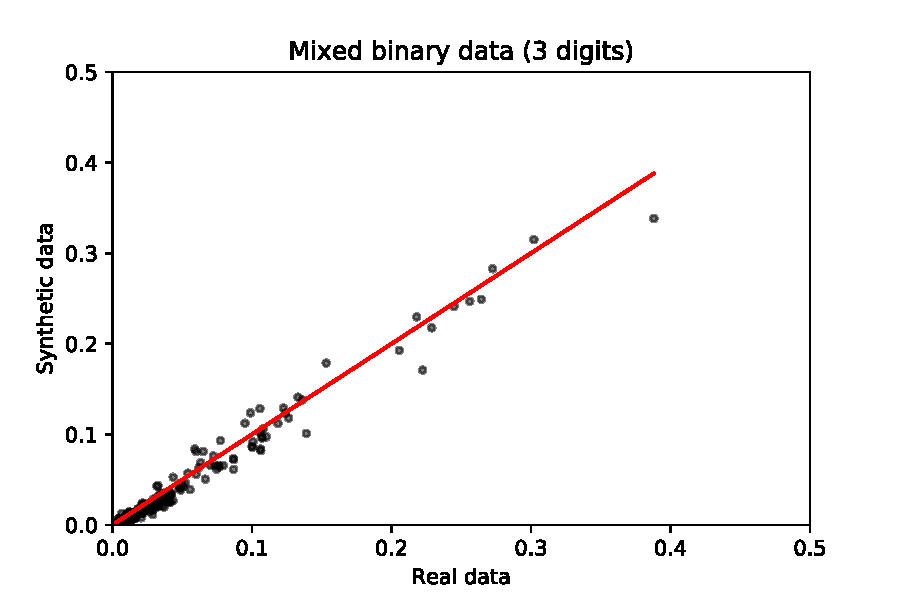
\includegraphics[width=.3\textwidth]{img/plots/binary_3digit_mixed}\hfill
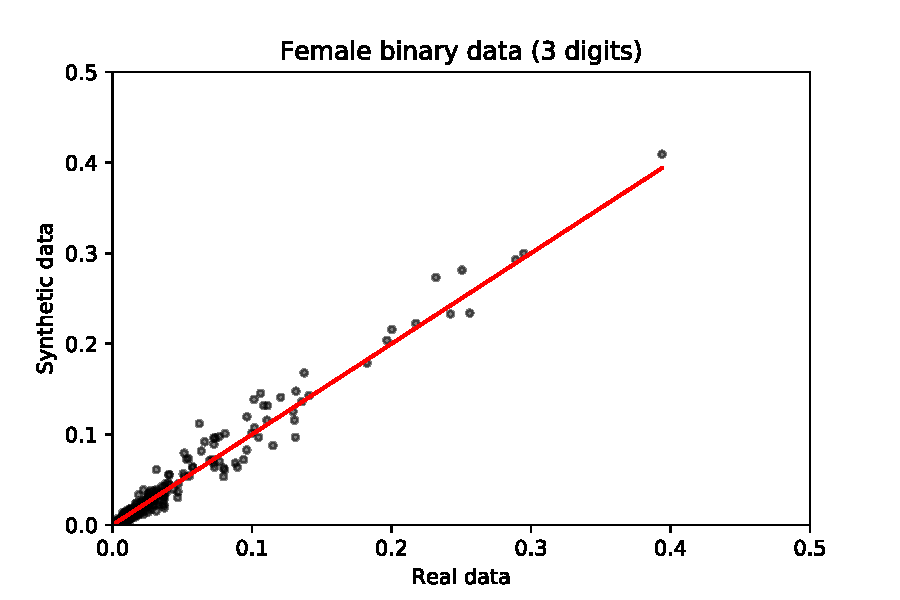
\includegraphics[width=.3\textwidth]{img/plots/binary_3digit_female}\hfill
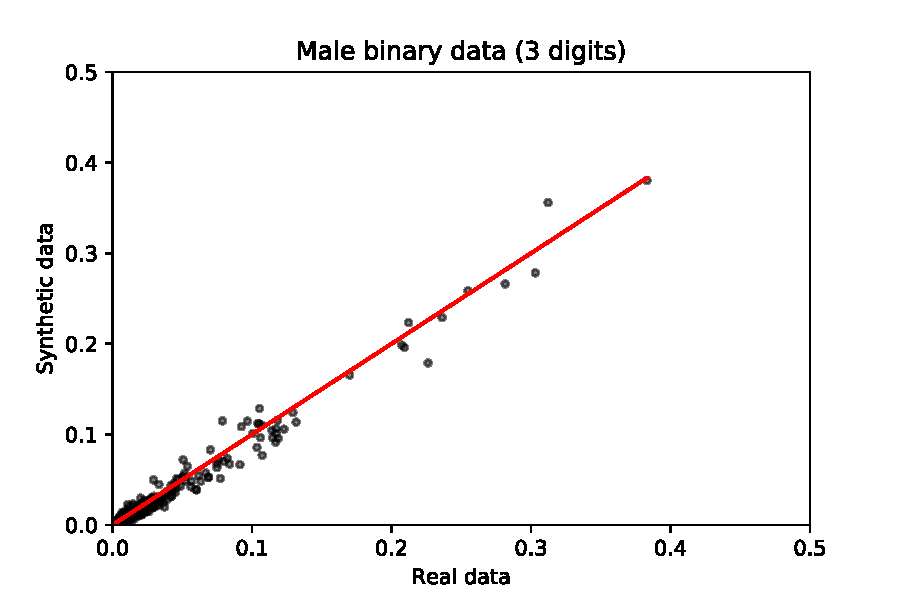
\includegraphics[width=.3\textwidth]{img/plots/binary_3digit_male}\hfill
\\
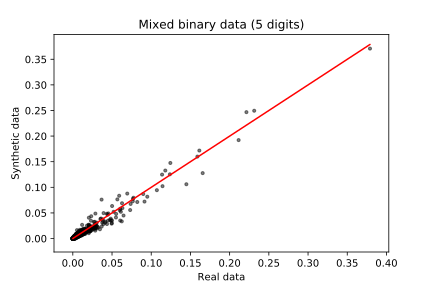
\includegraphics[width=.3\textwidth]{img/plots/binary_5digit_mixed}\hfill
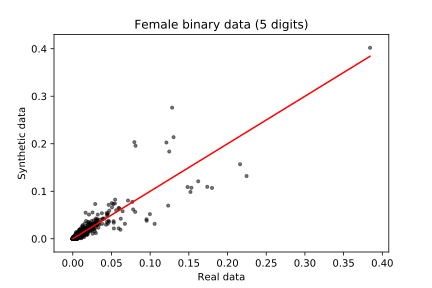
\includegraphics[width=.3\textwidth]{img/plots/binary_5digit_female}\hfill
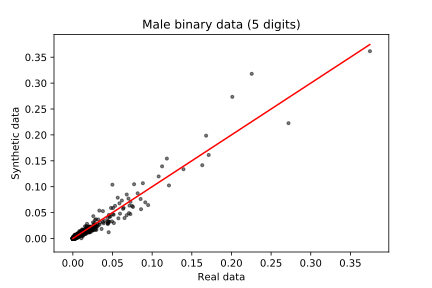
\includegraphics[width=.3\textwidth]{img/plots/binary_5digit_male}\hfill
\caption{Scatterplots of dimension-wise probability}
\begin{flushleft}
\end{flushleft}
\label{fig:figure3}
\end{figure}
Subsequently we will present our findings. In \textbf{Figure 5.1} we can see, after splitting up the dataset by gender, the performance decreased against our expectations for generating both, male and female samples, while male samples are not affected as heavily. In the best case scenario, all dots would accumulate along the regression line (red). However, we can see that the dots generated with the gender-specific models are more spread out than these for the model containing all data, meaning that the model did not learn the distribution as good as it did with the full input dataset.
 The performance loss for the models trained with 3 digits ICD-9 codes is still comparable to the performance with the original dataset. In comparison
\subsubsection{The performance of gender-based models decreased strongly for count data}
First, because the plots are more spread, we see that especially for count data, the performance decreased, when using gender-based models in comparison to using the full dataset. This affects the model trained with female samples more heavily than the model trained with male samples.

\subsubsection{The performance decreased slightly for binary data}
Second, we see that the performance loss for binary data is just slightly. The model trained with male samples performed better than the model trained with female samples. This seems to be due to the higher number of input data.


\textbf{Figure 5.2} depicts, that also for count variables, the performance decreased after splitting up the dataset. This especially affects the model, trained with female data only. This seems to be due to the same reasons as already mentioned for binary data.



\\
\\
\begin{figure}
\centering
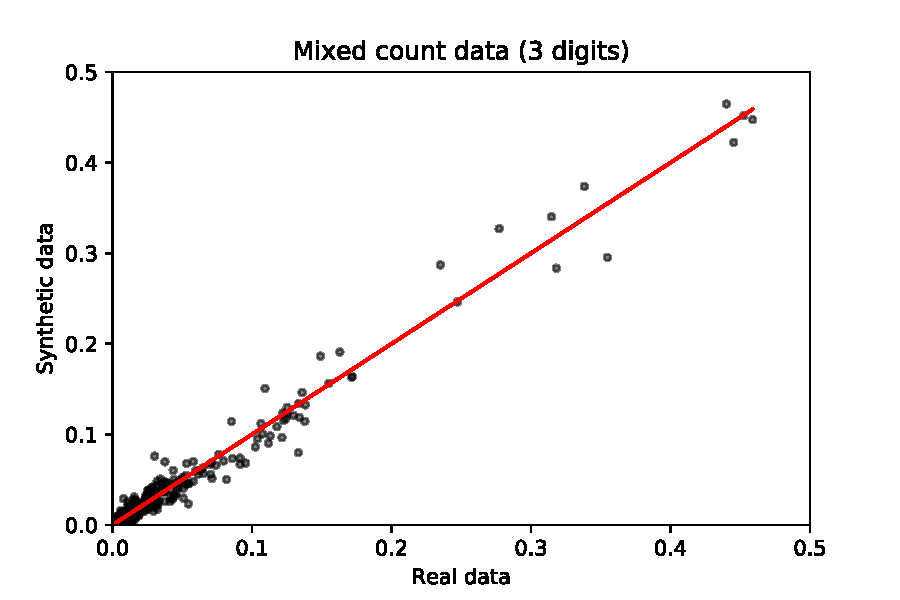
\includegraphics[width=.3\textwidth]{img/plots/count_3digit_mixed}\hfill
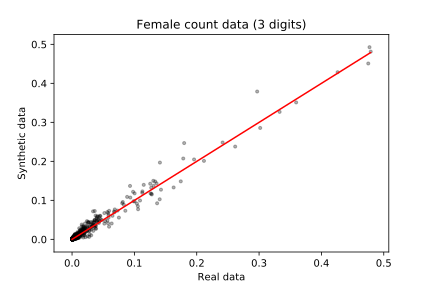
\includegraphics[width=.3\textwidth]{img/plots/count_3digit_female}\hfill
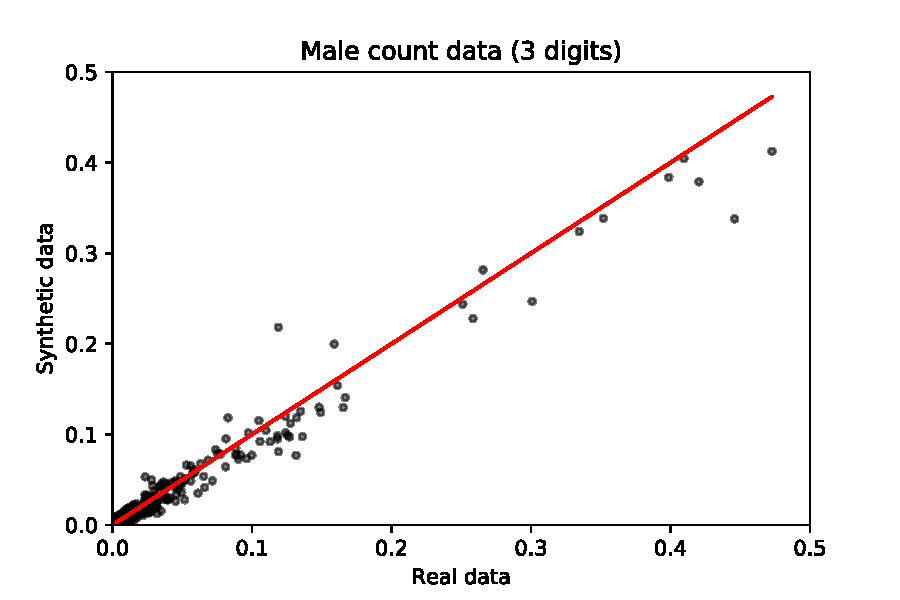
\includegraphics[width=.3\textwidth]{img/plots/count_3digit_male}\hfill
\\
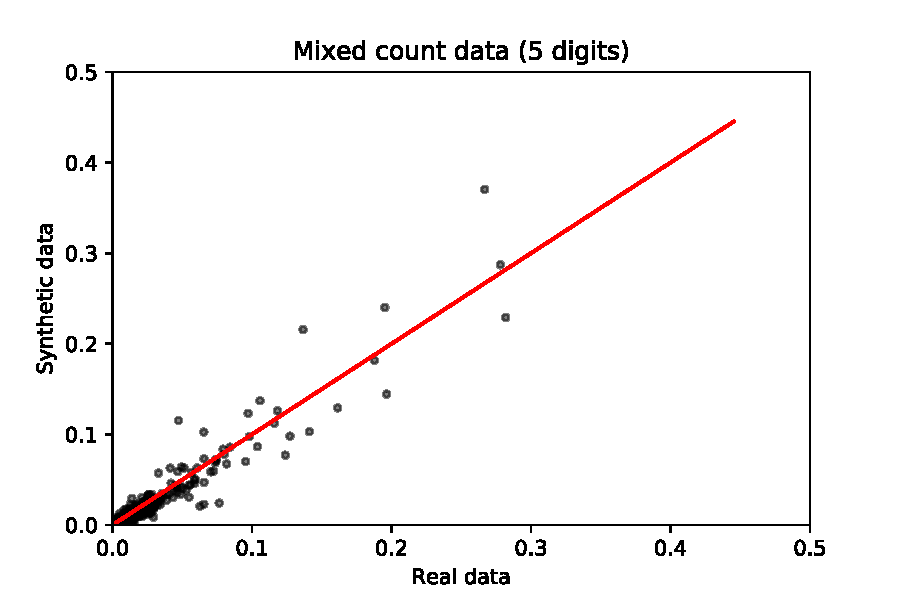
\includegraphics[width=.3\textwidth]{img/plots/count_5digit_mixed}\hfill
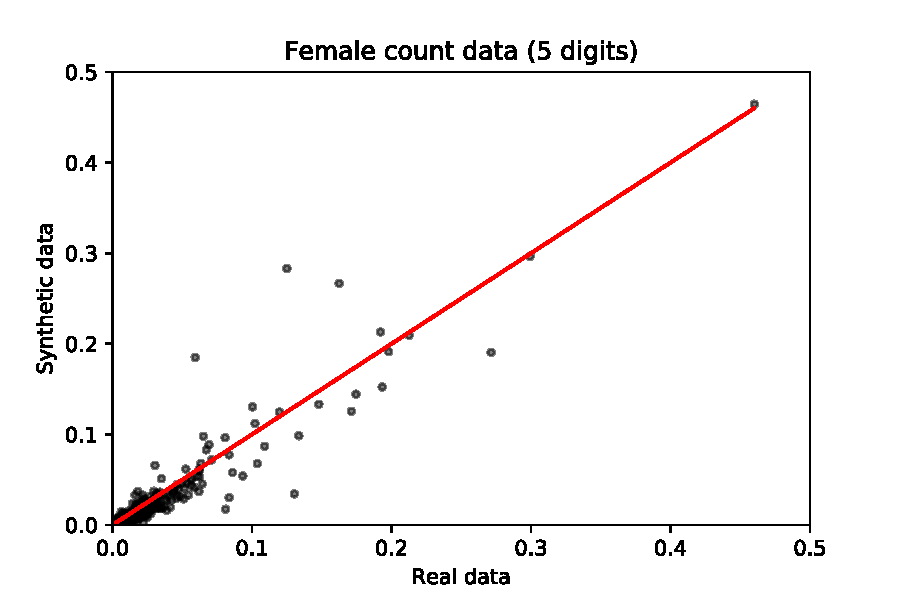
\includegraphics[width=.3\textwidth]{img/plots/count_5digit_female}\hfill
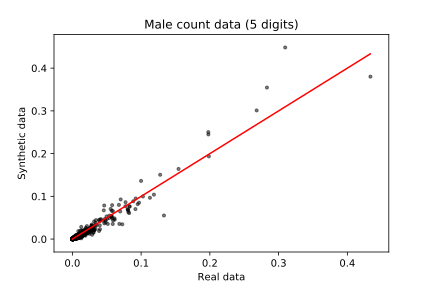
\includegraphics[width=.3\textwidth]{img/plots/count_5digit_male}\hfill
\caption{Scatterplots of dimension-wise average}
\begin{flushleft}
\end{flushleft}
\label{fig:figure3}
\end{figure}

\subsubsection{Evaluation Orphan diseases}
For evaluating our measurements for generated patients with rare diseases, we depict our results in a table with numbers of total occurrences, since we want to find out whether the model learns to generate them at all. First, we choose the binary data for evaluation. Second we will show the results for the count data.
For this case, the qualitative evaluation is of higher importance, since we have to find out whether the generated samples seem realistic to a medical doctor.


\textbf{Orphan diseases}:
\\
\\
\\
\begin{table}
\begin{center}
\begin{tabularx}{\textwidth}{X|r}
ICD-9 Code & No. of diagnoses\\
\hline
042 Human immunodeficiency virus [HIV] disease & 538\\
075 Infectious mononucleosis & 11\\
138 Late effects of acute poliomyelitis & 73 \\
193 Malignant neoplasm of thyroid gland & 49 \\
220 Benign neoplasm of ovary & 25\\
317 Mild intellectual disabilities & 82\\
515 Postinflammatory pulmonary fibrosis & 544\\
570 Acute and subacute necrosis of liver & 1067\\
8832 Open wound of finger(s), with tendon involvement & 17\\ 
\end{tabularx}
\end{center}
\caption{\label{tab:rare-MIMIC-III}rare disease diagnoses in MIMIC-III}
\end{table}

\begin{table}
\begin{tabularx}{\textwidth}{X|r|r}
ICD-9 Code & No. of diagnoses binary & No. of diagnoses count\\
\hline
042 Human immunodeficiency virus [HIV] disease	& 373 & 265\\
075 Infectious mononucleosis & 0 & 0\\
138 Late effects of acute poliomyelitis & 24  & 26\\
193 Malignant neoplasm of thyroid gland & 0 & 40\\
220 Benign neoplasm of ovary & 0 & 22\\
317 Mild intellectual disabilities & 0 & 22\\
515 Postinflammatory pulmonary fibrosis & 492 & 699\\
570 Acute and subacute necrosis of liver & 870 & 494\\
8832 Open wound of finger(s), with tendon involvement & 0 & 49\\ 
\end{tabularx}
\caption{\label{tab:rare-generated}successfully generated samples with rare diseases}
\end{table}
\\
After comparing the list of diagnoses of MIMIC-III with the list of Orphacodes from wikidata, we find 9 matching codes. Table 5.1 depicts the number of occurrences of each code in the original dataset. In \textbf{Table 5.2} we see, that our model successfully generates samples with 8 out of the 9 rare disease codes if we use count data. For binary data only 4 out of 9 codes are generated successfully. We can also see that neither the binary nor the count data model successfully generates samples with \texti{Infectious mononucleosis}, that only occurs 11 times in MIMIC-III. 
The count samples will be thoroughly evaluated by a medical doctor in our qualitative evaluation in the next section.


\subsection{Qualitative Evaluation}
Our qualitative evaluation consists of three parts. First, we repeat the steps of our data analysis and compare our synthetic samples with it. Second, we investigate whether the model learned gender-specific correlations of diseases and whether it learned to generate sample patients with rare diseases. This can be seen as a further test that proofs whether the model learned the interdimensional relationships. Third, we rate our measurements with the help of a medical doctor. Therefore we take 25 samples from the original dataset and 25 samples from our generated patients. Then, we present them in random order to a medical doctor and let him rate them on realisticness on a scale from 1 to 10, where 10 is the highest score and therefore a sample, that can not be distinguished from a real record.
The samples are selected randomly, except for the rare diseases. Here we choose 5 samples each from the dataset and from our generated patients because of their scarcity.

\subsubsection{Data analysis}

\begin{table}
\begin{tabular}{l|r}
\textbf{ICD-9 Code} & \textbf{Percent of affected patients}\\
\hline
401.9  Essential hypertension & 37.01\%\\
427.31 Atrial fibrillation & 24.68 \%\\
414.01 Coronary atherosclerosis & 22.81\%\\
428.0 Congestive heart failure & 19.22\%\\
272.4 unspecified hyperlipidemia & 17.18\%\\
250.00 Diabetes mellitus & 16 \%\\
599.00 Urinary tract infection & 14.75 \%\\
V29.0 suspected infectious condition of newborn & 13.27\%\\
584.9 Acute kidney failure & 12.77\%\\
V05.3 Need for prophylactic vaccination against viral hepatitis & 12.54\%\\
\end{tabular}
\caption{\label{tab:top10-icd-mixed}Top 10 diagnoses for generated samples (both sexes).}
\end{table}

\begin{table}
\begin{tabular}{l|r}
\textbf{ICD-9 Code} & \textbf{Percent of affected patients}\\
\hline
401.9  Essential hypertension & 20.47\%\\
427.31 Atrial fibrillation & 14.57\%\\
244.9 Unspecified acquired hypothyroidism & 11.92\%\\
305.1 Tobacco use disorder & 10.60\%\\
424.1 Aortic valve disorders & 9.68\%\\
414.01 Coronary atherosclerosis & 8.90\%\\
V58.1 Antineoplastic chemotherapy and immunotherapy & 8.70\%\\
V05.3 Need for prophylactic vaccination against viral hepatitis & 7.78\%\\
250.00 Diabetes mellitus & 7.45 \%\\
428.0 Congestive heart failure & 7.44\%\\
\end{tabular}
\caption{\label{tab:top10-icd-mixed}Top 10 diagnoses for generated samples (female).}
\end{table}

\begin{table}
\begin{tabular}{l|r}
\textbf{ICD-9 Code} & \textbf{Percent of affected patients}\\
\hline
401.9  Essential hypertension & 36.16\%\\
427.31 Atrial fibrillation & 31.79 \%\\
428.0 Congestive heart failure & 27.35\%\\
414.01 Coronary atherosclerosis & 22.25\%\\
584.9 Acute kidney failure & 19.85\%\\
272.4 unspecified hyperlipidemia & 16.12\%\\
V05.3 Need for prophylactic vaccination against viral hepatitis & 15.43\%\\
250.00 Diabetes mellitus & 14.14\%\\
V29.0 suspected infectious condition of newborn & 13.92\%\\
518.81  Acute respiratory failure & 13.37\%\\
\end{tabular}
\caption{\label{tab:top10-icd-mixed}Top 10 diagnoses for generated samples (male)}
\end{table}

We compare the Top 10 diagnoses of our generated samples \textbf{(Table 5.3)} to these of the original dataset \textbf{(Table 3.1)}. Most percentages are close to these of the original dataset but there are some outliers, for example Code 414.01 with a difference of 6.17% to the original dataset. This confirms our results from the quantitative evaluation.

\subsubsection{Gender-specific}
MedGAN as provided in its original form, already is, as stated by \cite{Choi2017}, able to generate patient EHR data, that can not be distinguished from real data by a medical doctor. The only exception is, when a patient's longitudinal record shows ICD-9 codes of both, female and male related diseases.  \cite{Choi2017}
By splitting up the input dataset into female and male patients, we eliminate this exception. Therefore we evaluate whether the data still seems real after dividing input data into two groups. For our Evaluation, we choose the binary dataset that has been generated by training with 5 digit long codes. The reason is, that we want to compare it with the results from Chapter 3, and for example the code for CAD (414.01) can not be identified by using only 3 digits,
First, as a basic check-up, we compare the top 10 occurring ICD-9 codes of our generated samples with those of the original dataset and look for any outliers. Subsequently, we check whether the model learned that female patients have an increased risk for coronary artery disease and cardiovascular disease, if they also have diabetic disease. 

Further, we put the focus of our examination on diabetic and ischemic diseases. 
From our generated samples, 1965 females are affected by both types, while 1689 males are affected by both. When generating patients, without separation 1501 are affected.
One of the known correlations is CAD (Cardiovascular Artery Disease) with Diabetes Mellitus. Women have an 3 to 6 fold increased risk if they have DM, while men have a 2 to 4 fold increased risk. \cite{juutilainen2004gender}
In our generated data 728 female patients, 907 male patients and 569 mixed patients are affected by DM.

\begin{table}
\begin{tabularx}{\textwidth}{X|r|r|r|r}
Gender & Affected by DM & Not affected by DM & Total & Percentage\\
\hline
Male 	& 2508 & 4973 & 7481 & 33.52/66.48\\
Female & 1143 & 1868 & 3011 & 37.96/62.04\\
\end{tabularx}
\caption{\label{tab:cad-diabetic-synth}Samples CAD diabetes / CAD no diabetes}
\end{table}

Looking at \textbf{Table 5.7} and \textbf{3.1} in comparison, we can see that the distribution for male and female samples with CAD and diabetes and these with no diabetes are similar. Therefore we conclude that the interdimensional relationship of cardiovascular disease with diabetic disease is not learned better, if we create gender-based models.

\subsubsection{Qualitative evaluation with a medical doctor}
Last, we evaluate our measurements with the help of a medical doctor. Therefore we choose 40 samples, 20 from the original dataset and 20 from our generated count datasets. For evaluation, we choose samples from the count dataset that we trained with 5 digit codes as input, as these are they best performing models according to our quantitative evaluation. From the samples with rare diseases, we choose 5 samples from the original dataset and 5 samples from the generated mixed dataset, again because of its superior performance . For the rest of the samples we choose 5 samples each, male, female, and mixed from the count datasets.
We ask the medical doctor to act as the discriminator for our samples, as already shown in \cite{Choi2017}. From the 40 presented, he rejected three.
One of the female samples, because it contained a code for chronic kidney disease and only one diagnosis for acute kidney failure, which is unlikely. One from the rare diseases samples, because a hypotension and a hypertension occurred together, which is highly unlikely. Another from the rare disease samples, got rejected because it had female-related and male-related codes.
Apart from these outliers, the samples are indistinguishable to a real record.


\subsection{Discussion}
% Risk Factors: do we see any changes in correlated illnesses from gender-specific to non gender-specific data?
% Qualitative: Doctor (note: A discussion with the doctor taught us that count data are easier to assess its realisticness than binary data. )
% Fragen, Ideen, Anregungen von Sait
A discussion with the medical doctor thought us that the evaluation of a patient's record on realistic-ness solely with diagnoses codes is a challenging task. The reason for this is that diseases are not mutually exclusive and every diagnosis is possible. Also generalization to 3 digit ICD codes is not helpful, because essential information about each diagnosis is lost. For example, shortening the ICD-9-CM Diagnosis Codes for a symptom like hallucinations (ICD-9 780.1) will only occur as 'General symptoms' (ICD-9 780) after generalization. 

\subsection{Summary}
In this chapter we evaluated our measurements in both, a quantitative and qualitative context. We learned from the quantitative evaluation, that separating the input data by gender does not improve the models performance in this context. The models trained with 3 digit ICD-9 codes outperformed those trained with 5 digit ICD-9 codes. Further the accuracy of the binary models is higher than the accuracy of the count models.
In our qualitative evaluation, a medical doctor rated the majority of the synthetic samples as real. In our discussion with him, we learned that using 3 digit codes generalizes diseases and symptoms to strongly and makes the samples hard to interpret.
This thought us that, while the 3 digit code models performed best in our quantitative evaluation, they are not superior in a qualitative manner.
\chapter{Conclusion and Outlook}
\section{Goal}
Our goal was to proof, that medGAN can generate realistic patients if it is trained with the MIMIC III dataset and that the model learns the distribution of ICD-9 codes. Further we tried to elaborate if by training the network with female and male patients separately, it is able to generate patients with gender-specific correlated diseases that seem realistic to a medical doctor. Also we wanted to find out whether the model is able to generate patients affected by orphan diseases that can not be distinguished to a non-synthetic patient by a medical doctor despite the rare occurrences in the dataset.
\section{Hypothesis proofed}
Our model successfully generates realistic patient data that can not be distinguished to real data, this also includes samples with rare diseases. However, the performance of medGAN did not increase after separating the input data by gender.
\section{Outlook}
Application to other MedGAN versions

\section{Future work}
Generating diagnosis and medication codes is the first step to generate high-quality synthetic EHR data. 
https://www.aclweb.org/anthology/W19-5026/
Problem: Utility of the data -> making it useful
Generating synthetic EHR data is the first step to replacing real training data. The next step  that would improve the utility of the samples could be the generation of clinical text with keyphrases. Our generated data could act as input data.

\section{Summary}
% approx. 0.5 pages
%wichtigste Punkte aus Discussion nochmal auflisten

\newpage

\section*{Acknowledgements}
I would like to express gratitude to Prof. Dr. Alexander Löser for the insightful discussions and valuable comments as well as his support and supervision of this thesis. I also would would like to express my gratitude to my advisor Betty van Aken for her continuous guidance and supervision. Further I want to thank Dr. med. Sait Subasi for evaluating the generated data. Without their help, this thesis would not have been possible.


\appendix
\renewcommand\chaptername{Appendix}

\chapter{Bibliography}

\chapter{Listings}
XXX

\chapter{Results} 
XXX






\end{document}
